\documentclass[10pt,a4paper]{article}
\usepackage[utf8]{inputenc} % para poder usar tildes en archivos UTF-8
\usepackage[spanish]{babel} % para que comandos como \today den el resultado en castellano
\usepackage{fullpage} %small margins
\usepackage[parfill]{parskip} %genera saltos entre parrafos
\usepackage{color}
\definecolor{gray}{gray}{0.35}
\usepackage{listings}
\usepackage{enumitem}
\usepackage{amsmath} %big brackets
\lstset{
    numbers=left,
    breaklines=true,
    tabsize=2,
    basicstyle=\ttfamily\color{gray},
}
\setlength{\parindent}{8pt}
\usepackage{mathtools}
\usepackage[margin=50pt]{geometry}
\usepackage{amsfonts}
\usepackage{flafter}
\usepackage{multicol}
\usepackage{subcaption}

\begin{document}

\section{Heurística de búsqueda local}
\subsection{Introduccion}

¿Qué es una \textbf{heurística de búsqueda local}? Una heurística de busqueda local, como su nombre indica, es un \textbf{procedimiento que busca, partiendo de una solución inicial $s$, una que sea mejor} que $s$ a través de "vecinos".

¿Qué son los vecinos de una solución? \textbf{Los vecinos de \boldmath{$s$}, denominados \boldmath{$N(s)$}} siendo $s$ una solución factible al problema, son aquellos que puedo \textbf{obtener realizando una modificación a \boldmath{$s$}}. Esa modificación es ad hoc al problema en sí, y, de hecho, la vecindad de una solución está definida por esa modificación. Por ejemplo, en k-PMP, si la vecindad está definida por tomar un nodo $v$ de un conjunto y colocarlo en otro conjunto, una solución $s$ tiene $s' \in N(s) \Leftrightarrow$ puedo obtener a $s'$ tomando un nodo $v$ de un conjunto y colocarlo en otro. Para esta vecindad, ocurre que $s \in N(s')$ ya que basta con colocar $v$ en su conjunto original.

¿Mejorar en cuánto a qué? Los problemas de \textbf{optimización combinatoria}, como el que es analizado en este trabajo práctico, son los cuáles se busca \textbf{optimizar una función \boldmath{$f:S\rightarrow \mathbb{R}$}}, donde $S$ es el conjunto de soluciones factibles para su correspondiente instancia $I$. La función $f$ para este problema es $f(s) =$ peso de solución $s$, con $s \in S$ para la instancia $I$ asociada. Por ende, \textbf{una solución \boldmath{$s'$} es mejor que una solución \boldmath{$s \Leftrightarrow f(s') < f(s)$}}. \textbf{La factibilidad de una solución está atada a reglas del problema}. Por ejemplo, en el k-PMP, una solución no puede distribuir menos nodos, en la partición, de los que tiene el grafo de entrada, tampoco podría describir una partición $P$ tal que $|P| > k$, etc.

¿Que nos detiene de \textbf{obtener la mejor solución}? \textbf{Encontrar la óptima es, efectivamente, resolver el problema}. La necesidad de tener heurísticas, de cualquier tipo, surge de \textbf{no conocer algoritmos que resuelvan la problemática en tiempo polinomial}, como es el caso del k-PMP. Por ende, buscamos algoritmos que nos permitan obtener soluciones ``buenas'' en un tiempo más razonable.

En particular, ¿por qué existen las busquedas locales? Dichas búsquedas proveen un servicio de \textbf{mejoramiento a otros algoritmos que generen soluciones}. Supongamos que una instancia $I$ fue puesta a través de un algoritmo heurístico goloso $HG$. Si esa instancia $I$ era particularmente mala para dicha heurística, la solución obtenida podría estar muy alejada de la óptima, que es lo que queremos tratar de evitar. Una buena idea es someter esa solución a un algoritmo de búsqueda local $HBL$ que atente a mejorarla. Al ser un algoritmo distinto, explora distintas posibilidades que la $HG$ no pudo ver.

¿\textbf{Siempre se puede llegar a una solución óptima de esta manera}? No siempre. \textbf{Si fuese así, tendríamos un algoritmo que resuelva el problema en tiempos razonables}. Por tiempos razonables nos referimos a tiempos no exponenciales, no podemos asegurar que siempre sean polinomiales ya que no toda heurística tiene una cota polinomial definida. Hasta puede ocurrir que para ciertas instancias sea imposible alcanzar el óptimo, por como fue definida vecindad, por como es la solución, o una mezcla de ambas. Hay heurísticas, denomidadas aproximadas, que tienen cotas de cuán mala puede ser la solución encontrada por dicho algoritmo. Sabiendo eso, si la cota no es muy holgada, combinar esa heurística con una de búsqueda local tendría altas probabilidades de generar muy buenas, o inclusive óptimas, soluciones. Pero, de nuevo, ni siquiera en esos casos podemos asegurar que siempre vamos a encontrar una óptima. \textbf{Esta es la razón por la cuál se denominan busquedas \textit{locales}}. \textbf{Buscan la mejor solucion, denominada óptimo local, en un conjunto \boldmath{$S'$} de soluciones tal que \boldmath{$S' \subseteq S$}, donde \boldmath{$S$} es el conjunto total de soluciones}, que depende de la solución inicial, de la vecindad planteada y de la instancia.

Habiendo dicho esto, \textbf{el procedimiento de la heurística de busqueda local es, dada una solución $s$, elegir el óptimo local $o$ dentro del conjunto $S' \subseteq S$ que forma la vecindad}. Entonces, esta solución $o$ es alguna una tal que $o \in S'$ y $f(o) \leq f(s')$, $\forall s' \in S'$, donde $f$ es la función a optimizar.

\newpage
\subsection{Busqueda Local 1}
\subsubsection{Desarrollo}
\noindent \textbf{\underline{Explicación de vecindad de la búsqueda local 1}}

El modo en que este algoritmo de búsqueda local va a operar es \textbf{revisando todos los vecinos de una solución y eligiendo el mejor}. Elegimos en el conjunto $S' = \left\{s\right\} \cup N(s)$ el óptimo local. Para toda solución $s$, la vecindad está definida por la siguiente función:

\textbf{\boldmath{$N1(s) =$} intercambiar un nodo \boldmath{$v$} en un conjunto, por otro nodo \boldmath{$u$} en otro conjunto distinto dentro la partición.}

En una solución $s$ genérica:

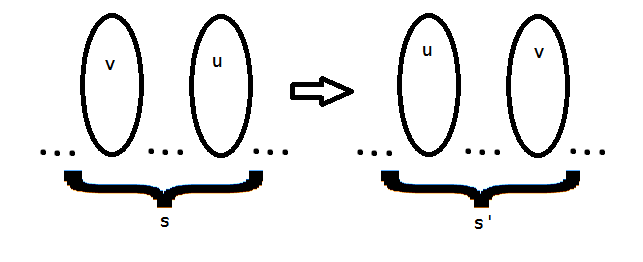
\includegraphics[scale=.75]{Vecindad1.png}

El tamaño de la vecindad depende de cuántos nodos puedo intercambiar, dejando de lado los nodos que estén en un mismo conjunto, ya que intercambiar 2 nodos dentro de un mismo conjunto deja el peso intrapartición intacto, por ende dejando el peso total intacto. En peor caso, en cuánto a cantidad de intercambios, podría pasar que todos los nodos estén en conjuntos distintos, por ende teniendo $(n-1)$ intercambios posibles para cada vértice, lo cuál genera un total $n*(n-1)$ posibles intercambios. Entonces, \textbf{para toda solución \boldmath{$s$}, \boldmath{$|N1(s)| \in O(n*(n-1)) = O(n^2)$}}. Esto nos dice que, \textbf{como mínimo, en peor caso, la función de complejidad temporal de dicho algoritmo debe ser de orden cuadrático en \boldmath{$n$} ya que esa es la cantidad de vecinos, como máximo, que podría tener una solución} y el algoritmo explora toda la vecindad.

\noindent \textbf{\underline{Pseudo código búsqueda local 1}}

\begin{lstlisting}
Solucion BusquedaLocal1(Grafo G = {v_1 ... v_n}, X), int k, Solucion s)
	Particion particion_actual = particion generada por s
	Particion mejor_particion = particion_actual
	para todo nodo v_i con i desde 1 a n:
		para todo nodo v_j con j desde 1 a n:
			si v_i esta en un conjunto distinto al v_j:
				colocar v_i en el conjunto donde se encuentra v_j dentro de la particion_actual
				colocar v_j en el conjunto donde se encontraba v_i dentro de la particion_actual
				si el peso total disminuyo:
					mejor_particion = particion_actual
				coloco v_i en su conjunto original dentro de la particion actual
				coloco v_j en su conjunto original dentro de la particion actual
				fin si
			fin si
		fin para
	fin para
	
	Solucion mejor_solucion = solucion asociada a la mejor_particion
	return mejor_solucion
\end{lstlisting}

Detalles a notar:
\begin{itemize}
\item No hace falta preguntar si $v_i \neq v_j$ ya que si están en conjuntos distintos, lo son.
\end{itemize}

\subsubsection{Complejidad}
\noindent \textbf{\underline{Comentarios preliminares}}
\begin{itemize}
\item Decidimos utilizar el código fuente para el cálculo de complejidad ya que brinda un cálculo más preciso y sin ambiguedades. Consideramos la línea 1 de un algoritmo como la línea donde, en el código fuente, se encuentra el return type, la declararción y los parámetros de una función.
\item Las estructuras utilizadas en el código son set y vector, ambas de la STL de c++.
\item Definimos \textit{Grafo} como vector\textless vector\textless float\textgreater \textgreater, \textit{Solución} como vector\textless int\textgreater, \textit{Conjunto} como set\textless int\textgreater y \textit{Partición} como vector\textless Conjunto\textgreater .
\end{itemize}

\noindent \textbf{\underline{La clase BusquedaLocal1}}

Decidimos colocar la heurística dentro de una clase llamada BusquedaLocal1 que consta de:

\textbf{Miembros privados de la clase}
\begin{itemize}
\item \textit{Solución solución\_inicial}: Contiene una copia de la solución a ser mejorada por la heurística.
\item \textit{Solución mejor\_vecino}: Contiene una copia del resultado de la heurística aplicada a la solución\_inicial o una copia de la solución\_inicial.
\item \textit{float peso\_mejor\_vecino}: Contiene el peso de mejor\_vecino si es que se usó previamente la función \textit{resolver}.
\end{itemize}

\textbf{Funciones relevantes públicas de la clase}
\begin{itemize}
\item \textit{Constructor BusquedaLocal1(const Solución}\& \textit{solución)}: Constructor que toma una solución como parametro y crea un objeto de la clase \textit{BusquedaLocal1} copiando la solución pasada como parámetro a \textit{solución\_inicia}l y a \textit{mejor\_vecino}. Operación que toma $O(n)$ dado que es copiar un vector de ints de tamaño $n$, y copiar un int tiene complejidad $O(1)$.
\item \textit{Solución resolver(const Grafo}\& \textit{grafo, int k, int n)}: Función que aplica la heurística de búsqueda local 1 a \textit{solución\_inicial}, almacenando el resultado en \textit{mejor\_vecino} y devolviéndolo. Complejidad analizada más abajo. \textbf{Esta función corresponde al pseudo código de la busqueda local 1 hecho más arriba.}
\item \textit{float getPeso()}: Función que devuelve peso\_mejor\_vecino. Complejidad $O(1)$.
\end{itemize}

\noindent \textbf{\underline{Complejidad algoritomo de BusquedaLocal1::resolver}}

\begin{itemize}
\item Líneas 2 - 3: 2 copias de objetos \textit{Partición}. Copiar un \textit{Conjunto} tiene complejidad $O(n)$, ya que en peor caso puede contener a todos los vértices, y hay $k$ conjuntos, por ende la complejidad es $O(2(n*k)) = O(n*k)$.
\item Líneas 3 - 18: \textit{For} que itera sobre la cantidad de nodos $\Rightarrow O(n * cuerpoFor1) = O(n^4 * k)$.
\item $cuerpoFor1$:
\begin{itemize}
\item Líneas 5 - 17: \textit{For} que itera sobre la cantidad de nodos $\Rightarrow O(n * cuerpoFor2) = O(n*n^2*k) = O(n^3 * k)$.
\item $cuerpoFor2$: 
\begin{itemize}
\item Línea 9: Complejidad de \textit{swapear\_nodos} $\in O(log(n))$ (Ver Complejidad Algoritmos Usados).
\item Línea 10: Compejidad de \textit{peso\_de\_partición} $\in O(n^2*k)$ (Ver Complejidad Algoritmos Usados).
\item Línea 11: Copia de una \textit{Partición} $\in O(n*k)$.
\item Línea 15: Complejidad de \textit{swapear\_nodos} $\in O(log(n))$ (Ver Complejidad Algoritmos Usados).
\end{itemize}
\item Complejidad $cuerpoFor2$ $\in O(n^2*k + n*k + log(n)) = O(n^2*k)$, por propiedades de la función $O$.
\end{itemize}
\item Complejidad $cuerpoFor1$ $O(1 + n^2*k) = O(n^3 * k)$, por propiedades de la función $O$.
\item Línea 19: Copiar un float $O(1)$ y Complejidad de \textit{peso\_de\_partición} $\in O(n^2*k)$ (Ver Complejidad Algoritmos Usados) $\Rightarrow \in O(n^2*k)$.
\item Línea 20: Copiar una \textit{Solución} tiene complejidad $O(n)$ y Complejidad de \textit{convertir\_particion\_en\_solucion} $\in O(n*k)$ (Ver Complejidad Algoritmos Usados) $\Rightarrow \in O(n + n*k) = O(n*k)$.
\item Línea 21: Devolver una \textit{Solución} por copia tiene complejidad $O(n)$.
\end{itemize}

\noindent \underline{Complejidad Total}: $O(n*k + n^4*k) = O(n^4*k)$ la cuál es pseudo-polinomial en el tamaño de la entrada.

Un pequeño análisis más en detalle de la complejidad nos muestra que lo que habíamos mencionado del tamaño de la vecindad es cierto. $O(n^3*k) = O((n^2)*(n^2*k))$, donde $O(n^2)$ es el costo de recorrer los vecinos y $O(n^2*k)$ es el costo de ``armar'' y obtener el valor de $f$, la función a optimizar, de cada vecino.

\textbf{\underline{Explicación y Complejidad Algoritmos Usados}}

\begin{itemize}
\item \textit{void swapear\_nodos(int nodo\_i, int conjunto\_nodo\_i, int nodo\_j, int conjunto\_nodo\_j, Partición}\& \textit{partición\_actual)}:
\begin{itemize}
\item Función que, dados los parámetros, toma el \textit{nodo\_i} y lo coloca en el \textit{conjunto\_nodo\_j}, y luego toma el \textit{nodo\_j} y lo coloca en el \textit{conjunto\_nodo\_j}.

\item Consta de 2 llamados de función de \textit{set::erase}, que tiene complejidad $O(log(n))$, y 2 llamados de función \textit{set::insert}, que también posee complejidad $O(log(n))$, con $n$ la cantidad de elementos del \textit{set}\newline $\Rightarrow \in O(4*log(n)) = O(log(n))$.
\end{itemize}
\item \textit{float peso\_de\_particion(Partición}\& \textit{partición, int k, Grafo}\& \textit{grafo))}:
\begin{itemize}
\item Función que, dado el \textit{Grafo} correspondiente, devuelve el peso total de la \textit{Partición} pasada como parámetro.
\item Consta de un \textit{For} que itera sobre $k$ donde cada iteración tiene un \textit{For} que itera sobre el tamaño del \textit{Conjunto}, denominado $n$, con un ciclo dentro que itera sobre el tamaño del conjunto, realizando operaciones con costo temporal $O(1)$ $\Rightarrow$ la complejidad de la función es $O(k*n*n*1) = O(n^2*k)$.
\end{itemize}
\item \textit{Solución convertir\_particion\_en\_solucion(Partición}\& \textit{partición, int k}):
\begin{itemize}
\item Función que transforma una \textit{Partición} en una \textit{Solución} válida.
\item Consta de un \textit{For} que itera tantas veces como $k$ que contiene otro \textit{For} que itera sobre $n$, la cantidad de elementos del \textit{Conjunto}, realizando operaciones de complejidad constante $\Rightarrow \in O(n*k)$.
\end{itemize}
\end{itemize}

\textbf{\underline{Costo total de aplicar la heurística sobre una solución}}

\begin{itemize}
\item Tomar el input (no se tiene en cuenta en el cálculo de Complejidad).
\item Creación del objeto \textit{BusquedaLocal1} con la solución a mejorar $\in O(n)$.
\item Llamado a \textit{BusquedaLocal1::resolver} sobre ese objeto $\in O(n^4*k)$.
\end{itemize}

\underline{Complejidad Total}: $O(n^4*k)$.

\newpage
\subsection{Busqueda Local 2}
\subsubsection{Desarrollo}
\noindent \textbf{\underline{Explicación de vecindad de la búsqueda local 2}}

El modo en que este algoritmo de búsqueda local va a operar es \textbf{revisando todos los vecinos de una solución y eligiendo el mejor}. Elegimos en el conjunto $S' = \left\{s\right\} \cup N(s)$ el óptimo local. Para toda solución $s$, la vecindad está definida por la siguiente función:

\textbf{\boldmath{$N2(s) =$ colocar un nodo $v$ en un conjunto distinto al que pertenece dentro de la partición.}}

En una solución $s$ genérica:

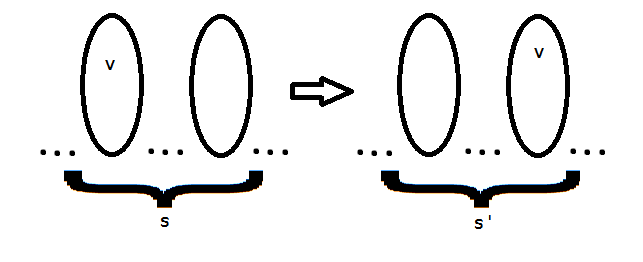
\includegraphics[scale=.75]{Vecindad2.png}

El tamaño de esta vecindad depende de en cuántos conjuntos distintos dentro de la partición puedo colocar a un vértice, y eso es siempre $(k-1)$, todos los conjuntos menos el mismo al que pertenece. Esto es cierto para todo vértice, \textbf{\boldmath{entonces para toda solución $s$ se cumple que $|N2(s)| = O(n*(k-1)) = O(n*k)$}}. Como para la anterior búsqueda local, se debe cumplir que el \textbf{\boldmath{algoritmo, como mínimo, perteneza a $O(n*k)$ dado que el algoritmo revisa toda la vecindad en busca del mejor vecino}}.

\noindent \textbf{\underline{Pseudo código de la búsqueda local 2}}

\begin{lstlisting}
Solucion BusquedaLocal1(Grafo G = {v_1 ... v_n}, X), int k, Solucion s)
	Particion particion_actual = particion generada por s
	Particion mejor_particion = particion_actual
	para todo nodo v_i con i desde 1 a n:
		para todo conjunto c_j desde 1 hasta k:
			si el nodo v_i no pertenece al conjunto c_j
				quitar v_i de su conjunto actual
				colocar v_i en el conjunto c_j
				si el peso total disminuyo:
					mejor_particion = particion_actual
				quitar v_i de c_j
				colocar v_i en su conjunto original correspondiente
				fin si
			fin si
		fin para
	fin para
	
	Solucion mejor_solucion = solucion asociada a la mejor_particion
	return mejor_solucion
\end{lstlisting}

\subsubsection{Complejidad}

\noindent \textbf{\underline{Comentarios preliminares}}
\begin{itemize}
\item Decidimos utilizar el código fuente para el cálculo de complejidad ya que brinda un cálculo más preciso y sin ambiguedades. Consideramos la línea 1 de un algoritmo como la línea donde, en el código fuente, se encuentra el return type, la declararción y los parámetros de una función.
\item Las estructuras utilizadas en el código son set y vector, ambas de la STL de c++.
\item Definimos \textit{Grafo} como vector\textless vector\textless float\textgreater \textgreater, \textit{Solución} como vector\textless int\textgreater, \textit{Conjunto} como set\textless int\textgreater y \textit{Partición} como vector\textless Conjunto\textgreater .
\end{itemize}

\noindent \textbf{\underline{La clase BusquedaLocal2}}

Decidimos colocar la heurística dentro de una clase llamada \textit{BusquedaLocal2} que consta de:

\textbf{Miembros privados de la clase}
\begin{itemize}
\item \textit{Solución solución\_inicial}: Contiene una copia de la solución a ser mejorada por la heurística.
\item \textit{Solución mejor\_vecino}: Contiene una copia del resultado de la heurística aplicada a la solución\_inicial o una copia de la solución\_inicial.
\item \textit{float peso\_mejor\_vecino}: Contiene el peso de mejor\_vecino si es que se usó previamente la función \textit{resolver}.
\end{itemize}
\textbf{Funciones relevantes públicas de la clase}
\begin{itemize}
\item \textit{Constructor BusquedaLocal1(const Solución}\& \textit{solución)}: Constructor que toma una solución como parametro y crea un objeto de la clase \textit{BusquedaLocal1} copiando la solución pasada como parámetro a \textit{solución\_inicia}l y a \textit{mejor\_vecino}. Operación que toma $O(n)$ dado que es copiar un vector de ints de tamaño $n$, y copiar un int tiene complejidad $O(1)$.
\item \textit{Solución resolver(const Grafo}\& \textit{grafo, int k, int n)}: Función que aplica la heurística de búsqueda local 1 a \textit{solución\_inicial}, almacenando el resultado en \textit{mejor\_vecino} y devolviéndolo. Complejidad analizada más abajo. \textbf{Esta función corresponde al pseudo código de la busqueda local 2 hecho más arriba.}
\item \textit{float getPeso()}: Función que devuelve peso\_mejor\_vecino. Complejidad $O(1)$.
\end{itemize}

\noindent \textbf{\underline{Complejidad algoritomo de BusquedaLocal2::resolver}}

\begin{itemize}
\item Líneas 2 - 3: Líneas 2 - 3: 2 copias de objetos \textit{Partición}. Copiar un \textit{Conjunto} tiene complejidad $O(n)$, ya que en peor caso puede contener a todos los vértices, y hay $k$ conjuntos, por ende la complejidad es $O(2(n*k)) = O(n*k)$.
\item Líneas 3 - 18: \textit{For} que itera sobre la cantidad de nodos $\Rightarrow O(n * cuerpoFor1) = O(n*(n^2*k^2)) = O(n^3*k^2) $
\item \textit{cuerpoFor1}:
\begin{itemize}
\item Líneas 4 - 16: \textit{For} que itera sobre la cantidad de conjuntos $\Rightarrow O(k * cuerpoFor2) = O(k*(n^2*k)) = O(n^2*k^2)$
\item \textit{cuerpoFor2}
\begin{itemize}
\item Línea 8: Complejidad de operación \textit{mover\_nodos} $\in O(log(n))$ (Ver Complejidad Algoritmos Usados).
\item Línea 9: Compejidad de \textit{peso\_de\_partición} $\in O(n^2*k)$ (Ver Complejidad Algoritmos Usados).
\item Línea 10: Copia de una \textit{Partición} $\in O(n*k)$.
\item Línea 14: Complejidad de operación \textit{mover\_nodos} $\in O(log(n))$ (Ver Complejidad Algoritmos Usados).
\end{itemize}
\item Complejidad \textit{cuerpoFor2} $\in O(n^2*k + n*k + 2log(n)) = O(n^2*k)$.
\end{itemize}
\item Complejidad \textit{cuerpoFor1} $\in O(n^2*k^2)$.
\item Línea 20: Copiar un float $O(1)$ y Complejidad de \textit{peso\_de\_partición} $\in O(n^2*k)$ (Ver Complejidad Algoritmos Usados) $\Rightarrow \in O(n^2*k)$.
\item Línea 21: Copiar una \textit{Solución} tiene complejidad $O(n)$ y Complejidad de \textit{convertir\_particion\_en\_solucion} $\in O(n*k)$ (Ver Complejidad Algoritmos Usados) $\Rightarrow \in O(n + n*k) = O(n*k)$.
\item Línea 22: Devolver una \textit{Solución} por copia tiene complejidad $O(n)$.
\end{itemize}

\underline{Complejidad Total}: $O(n^3*k^2)$.

Un pequeño análisis más en detalle de la complejidad nos muestra que lo que habíamos mencionado del tamaño de la vecindad es cierto. $O(n^2*k^2) = O((n*k)*(n^2*k))$, donde $O(n*2)$ es el costo de recorrer los vecinos y $O(n^2*k)$ es el costo de ``armar'' y obtener el valor de $f$, la función a optimizar, cada vecino.

\textbf{\underline{Explicación y Complejidad Algoritmos Usados}}

\begin{itemize}
\item \textit{void mover\_nodos(int nodo\_i, int conjunto\_nodo\_i, int conjunto\_j, Partición}\& \textit{partición\_actual)}:
\begin{itemize}
\item Función que, dados los parámetros, toma el \textit{nodo\_i} y lo coloca en el \textit{conjunto\_j}, y luego quita el \textit{nodo\_i} del \textit{conjunto\_nodo\_i}.
\item Consta de 1 llamado a la función de \textit{set::erase}, que tiene complejidad $O(log(n))$, y 1 llamado a la función \textit{set::insert}, que también posee complejidad $O(log(n))$, con $n$ la cantidad de elementos del \textit{set} $\Rightarrow \in O(2*log(n)) = O(log(n))$.
\end{itemize}
\item \textit{float peso\_de\_particion(Partición}\& \textit{partición, int k, Grafo}\& \textit{grafo))}:
\begin{itemize}
\item Función que, dado el \textit{Grafo} correspondiente, devuelve el peso total de la \textit{Partición} pasada como parámetro.
\item Consta de un \textit{For} que itera sobre $k$ donde cada iteración tiene un \textit{For} que itera sobre el tamaño del \textit{Conjunto}, denominado $n$, con un ciclo dentro que itera sobre el tamaño del conjunto, realizando operaciones con costo temporal $O(1)$ $\Rightarrow$ la complejidad de la función es $O(k*n*n*1) = O(n^2*k)$.
\end{itemize}
\item \textit{Solución convertir\_particion\_en\_solucion(Partición}\& \textit{partición, int k}):
\begin{itemize}
\item Función que transforma una \textit{Partición} en una \textit{Solución} válida.
\item Consta de un \textit{For} que itera tantas veces como $k$ que contiene otro \textit{For} que itera sobre $n$, la cantidad de elementos del \textit{Conjunto}, realizando operaciones de complejidad constante $\Rightarrow \in O(n*k)$.
\end{itemize}
\end{itemize}

\textbf{\underline{Costo total de aplicar la heurística sobre una solución}}

\begin{itemize}
\item Tomar el input (no se tiene en cuenta en el cálculo de Complejidad).
\item Creación del objeto \textit{BusquedaLocal1} con la solución a mejorar $\in O(n)$.
\item Llamado a \textit{BusquedaLocal1::resolver} sobre ese objeto $\in O(n^3*k^2)$.
\end{itemize}

\underline{Complejidad Total}: $O(n^3*k^2)$.

\newpage
\subsection{Experimentacion}

\noindent \textbf{\underline{Análisis de Calidad}}

\noindent \textbf{Medición de calidad con Solución Greedy}

Para esta medición, \textbf{generamos instancias con \boldmath{$k < n$}} ya que el algoritmo greedy devuelve una respuesta exacta en caso contrario. Si $k \geq n$, basta con colocar un nodo por conjunto y obtenemos una solución óptima con peso $0$. Veamos el gráfico de dichas mediciones:

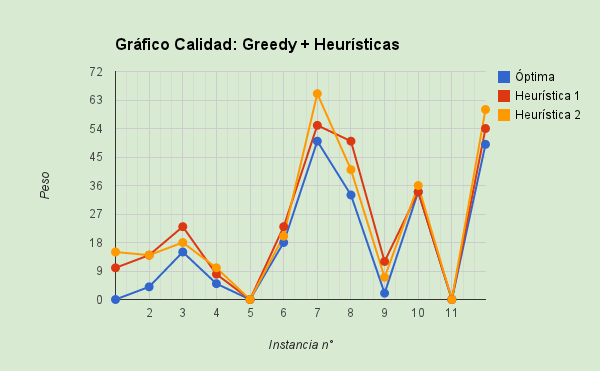
\includegraphics[scale=0.45]{grafico_calicad_greedy_heuristicas.png}

\textbf{En estas condiciones, ninguno es claro vencedor. Esto puede deberse al hecho de que las vecindades son ``similares'' en cuánto a cómo son sus vecinos}, realizar un intercambio de nodos entre 2 conjuntos distintos es lo mismo que tomar un nodo, colocarlo en un conjunto y luego tomar otro nodo distinto y colocarlo en el conjunto donde se encontraba el vértice anteriormente mencionado. 

Lo que si se puede apreciar del gráfico es que las soluciones obtenidas por las heurísticas no son excesivamente lejanas a las óptimas. Dicho fenómeno no ocurre espontáneamente, \textbf{mientras mejor es la solución inical, la solución encontrada por la heurística también lo va a ser.} Formalmente, la respuesta de una heurística, a lo sumo, es igual de buena a la solución inicial, nunca peor, sino caería fuera de la definición de heurística. En consecuencia, tener buenas soluciones iniciales favorece que la heurística acabe en una buena solución final.

\noindent \textbf{Medición de calidad con Solución Aleatoria}

El siguiente gráfico muestra \textbf{instancias sin ningún tipo de particularidad}. La diferencia con el caso anterior es que, inclusive con $k \geq n$, como la solución es generada al azar, no necesariamente la solución obtenida es óptima. Por eso, en estas condiciones, es relevante analizar todos los casos, y no restringirlo a $k < n$.

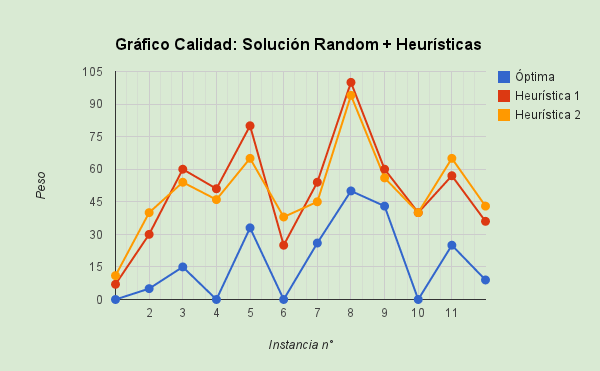
\includegraphics[scale=0.45]{grafico_calicad_greedy_random.png}

Como en el análisis de calidad anterior, \textbf{ninguno de los 2 se destaca claramente.} Por otra parte, es claro que \textbf{las heurísticas entregaron soluciones peores que las del análisis previo}. Las soluciones aleatorias pueden ser excesivamente malas, inclusives las peores, y eso se ve reflejado en los resultados obtenidos. Es fácil ver que, para estas heurísticas, \textbf{siempre conviene tener inicialmente una solución púlida.} Por esto es que, en la introducción a esta sección del trabajo práctico, mencionamos que las \textbf{heurísticas de búsqueda local brindan un servicio de complemento a otros algoritmos, incluyendo heurísticas, de generación de soluciones.} 
\newpage

\noindent \textbf{\underline{Análisis de Tiempos}}

\noindent \textbf{Metodología de medición}

Para cada tamaño n, generamos 100 instancias. Luego, para cada instancia, medimos su tiempo de ejecución 50 veces, quedándonos con la ejecución que menor tiempo tomo. Finalmente, obtuvimos un promedio de esos valores y el resultado de dicha operación es la que fue colocada en los gráficos. Tomamos el mínimo de cada instancia debido a que el procesador atiende varios procesos en simultáneo y, por ende, es díficil obtener un valor fiel de cuánto realmente toma ejecutar el algoritmo sobre la instancia actual. Tomando el mínimo eliminamos la mayor cantidad de tiempo gastado en operaciones fuera de la ejecución de nuestro algoritmo.

\noindent \textbf{Medición de tiempos}

Ya que ambos algoritmos dependen, en cuánto a complejidad temporal, de $k$, una variable que no tiene relación directa con el tamaño de la entrada $n$, decidimos realizar un análisis de tiempos variando el $k$, esto fue lo que obtuvimos:

\begin{figure}[h!]
\begin{subfigure}{0.5\textwidth}
	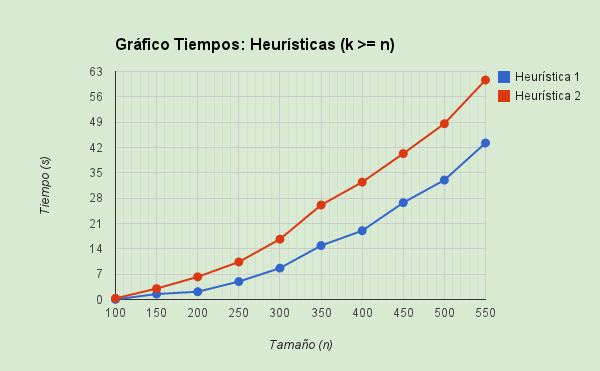
\includegraphics[width=\textwidth, height=60mm]{grafico_tiempos_heuristicas_kmayorigualn.png}
\end{subfigure}
\begin{subfigure}{0.5\textwidth}
	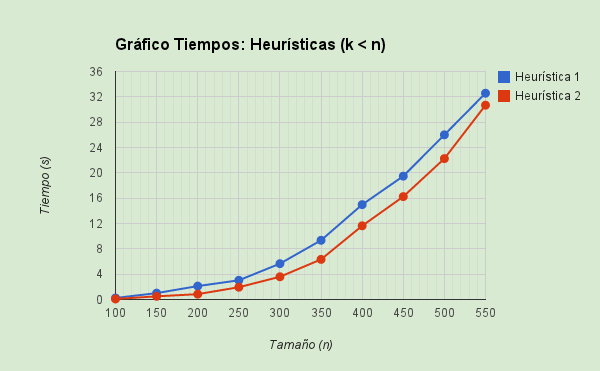
\includegraphics[width=\textwidth, height=60mm]{grafico_tiempos_heuristicas_kmenorn.png}
\end{subfigure}
\end{figure}

\textbf{Los resultados son coherentes al análisis de complejidad hecho anteriormente, el algoritmo 2 está más atado al $k$ que su contraparte}. Pero, conceptualmente, \textbf{¿Cuál es la razón?} Ya habíamos mencionado \textbf{el tamaño de la vecindad de cada heurística: para la 1 el tamaño \boldmath{$\in O(n^2)$} y para la 2da \boldmath{$\in O(n*k)$}}. Si $k < n$, la vecindad de la segunda heurística tiene una cota más ajustada de $O(n^2)$, por eso las mediciones son similares para dicho caso. En cambio, si $k \geq n$, ninguna se tiene una cota mejor. Si bien $O(n^2) = O(n^k)$, para este caso, eso no significa que la vecindad de la heurística 1 depende de $k$, nada más es una cota más ``grosera'' que no refleja el comportamiento adecuadamente. Veamos el siguiente caso: $n = 5$ y $k = 100$, está claro que la vecindad 2 va a ser más numerosa que la 1, independientemente de los pesos de las aristas y de la densidad del grafo. Inclusive, \textbf{uno podría tener un $k$ tan alejado de $n$ como quisiera y así obtener costos temporales potencialmente caros}. 

\textbf{De todas formas, poseemos un algoritmo polinomial que otorga una solución óptima para casos tales que \boldmath{$k \geq n$}} y esa información no es costosa de obtener, se pregunta si eso ocurrre, en $O(1)$, inmediatamente luego de tomar el input. Por lo cuál no habría que preocuparse demasiado por este tipo de casos.

\end{document}